\documentclass{article}

\usepackage{amsmath, amsthm, amssymb, amsfonts}
\usepackage{thmtools}
\usepackage{graphicx}
\usepackage{setspace}
\usepackage{geometry}
\usepackage{float}
\usepackage{hyperref}
\usepackage[utf8]{inputenc}
\usepackage[english]{babel}
\usepackage{framed}
\usepackage[dvipsnames]{xcolor}
\usepackage{tcolorbox}
\usepackage{enumitem}
\usepackage{tikz}
\usepackage{tikz-3dplot}
\usepackage{graphicx}
\usepackage{biblatex}

\addbibresource{bibliography.bib}

% \colorlet{LightGray}{White!90!Periwinkle}
\colorlet{LightGray}{Blue!30}
\colorlet{LightOrange}{Orange!15}
\colorlet{LightGreen}{Green!15}

\newcommand{\HRule}[1]{\rule{\linewidth}{#1}}

\declaretheoremstyle[name=Theorem,]{thmsty}
\declaretheorem[style=thmsty,numberwithin=section]{theorem}
\tcolorboxenvironment{theorem}{colback=LightGray}

\declaretheoremstyle[name=Proposition,]{prosty}
\declaretheorem[style=prosty,numberlike=theorem]{proposition}
\tcolorboxenvironment{proposition}{colback=LightOrange}

\declaretheoremstyle[name=Principle,]{prcpsty}
\declaretheorem[style=prcpsty,numberlike=theorem]{principle}
\tcolorboxenvironment{principle}{colback=LightGreen}


\makeatletter
\renewcommand{\maketitle}{%
  \begin{center}
    \vspace*{3cm} % Adjust the vertical space as needed
    {\LARGE\@author\par}
    \vspace{1cm} % Adjust the vertical space as needed
    {\Huge\bfseries\@title\par}
    \vspace{2cm} % Adjust the vertical space as needed
    {\Large\@date\par}
  \end{center}
}
\makeatother


\begin{document}

\title{ \normalsize \textsc{}
\\ [0.5cm]
\HRule{1.0pt} \\
\Huge \textbf{The Evasion Problem}
\HRule{1.0pt}
\\ [1.5cm]
\LARGE{Andrej Jočić \\ Matija Ojo}
}
\author{\textbf{Computational Topology - group project}}
\date{\today}

\maketitle

\newpage


\section{Introduction}

The evasion problem asks if there is a way to move in an area, covered with moving sensors, and not be detected.
We assume the sensors follow a predefined path and their movement is periodic.
This means that, after some period, the area covered by sensors is identical.
Furthermore, we assume the area in question is a subspace of the plane $ \mathbb{R}^2 $.
These assumptions do not lose generality, since movement of real sesnors is often periodic and movement through an area can be modelled in the plane.

This solution could be applied to the problem of determining the optimal amount of sensors and their paths to cover the area.
The goal in this case is not to cover the entire area at all times, but to cover parts of it with fewer sensors, such that a potential intruder cannot avoid detection throughout the whole period.

The following are additional assumptions taken into account, which do lose on generality, however greatly simplify the implementation:
\begin{itemize}
  \item the intruder's movement speed is unbounded,
  \item the area in question is a rectangular grid,
  \item the paths along which the sensors move are straight line segments,
  \item all sensors move at the same speed of one unit of distance per one unit of time,
  \item each sensor covers a square area two units of distance across oriented parallel to the edges of the room they protect.
\end{itemize}


\section{Methods}

By considering the area not covered by the senors (two-dimensional object) at each point in time $t \in \mathbb{R}$, we obtain a three-dimensional (free) complex $F$ embedded in space-time.
We are only interested in the times up to the (global) sensor network period $p$, since the object simply repeats itself after $p$.
Therefore, the complex we obtain is similar to a torus, where the first point in time is ``glued'' to the time at $t = p$.
One way to obtain the evasion paths would be to compute $ H_1 (F, \mathbb{Z}) $ and check which generators represent vaild cycles/paths (i.e. cycles going strictly forward in time).
However, we decided to take a different approach and collapse the free complex to a directed graph and compute cycles from the starting nodes of the graph.

\subsection{Sensors}

Since all the sensors have the same properties (area covered, speed of movement), they are only defined by the \texttt{Path} which they follow.
A \texttt{Path} is a sequence of \texttt{Position}s, where a \texttt{Position} is point in the plane $(x, y)$.
Since we want the sensors to move along straight line segments, two consecutive \texttt{Position}s need to either have the same $x$ or $y$ coordiantes.
The length of a \texttt{Path} is the sum of all the consecutive line segments that form it.
Sensors move towards the next defined \texttt{Position} in the \texttt{Path}, and move towards the first \texttt{Position} when reaching the last one.

The \texttt{SensorNetwork} class is a collection of \texttt{Sensor}s along with the width and height of the rectangular area.
\texttt{SensorNetwork} represents the entire configuration of the input, since the behaviour of the system is determined by the initial situation.
The global period of the system ($p$) is the least common multiple of all the sensor \texttt{Path}'s lengths.

\subsection{Free complex}

For the data structure of the free complex ($F$), we used the \href{https://gudhi.inria.fr/python/latest/cubical_complex_user.html}{\texttt{CubicalComplex}} from the \href{https://pypi.org/project/gudhi/}{gudhi} library.
This approach is the simplest, because the area covered by each sensor is a square (ie. a 2-dimensional simplex, defined by 4 points), so we do not have to do any transformation.

We can even further simplify the complex construction, by not taking any wedge shapes into account.
A wedge shape is a situation where a cell in the grid was covered at time $t$, but is not covered at time $t + 1$ or vise versa - not covered at $t$, covered at $t + 1$.
In a 3-dimensional cubical complex that would result in a wedge.
We can omit those shapes, because the object trying to avoid detection can either be in a particular cell or not - we do not allow partially taking halves of 2 cells.
Therefore, the valid positions for the object, trying to avoid detection, are only those, which are not covered at two consecutive times.
If we consider the case where the cell was covered at time $t$ and was not covered at time $t + 1$ and take a look at the complex from the top-down perspective, we would obtain something like this:

\smallskip

\begin{figure}[H]
  \centering

  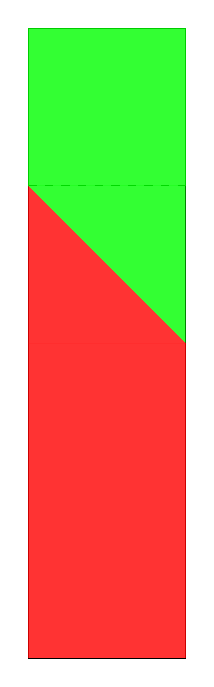
\begin{tikzpicture}[scale=2,transform shape]
    \draw (0,0) rectangle (1,4);
    \draw[dashed] (0,3) -- (1, 3);

    \fill[red, opacity=0.8] (0,0) rectangle (1, 2.001);
    \fill[red, opacity=0.8] (0, 2) -- (1, 2) -- (0, 3) -- cycle;
    \fill[green, opacity=0.8] (1,2) -- (1,3) -- (0,3) -- cycle;
    \fill[green, opacity=0.8] (0, 3) rectangle (1, 4);
  \end{tikzpicture}

  \caption{Top-down representation of a wedge shape in a cubical complex.}
  \label{fig:wedge}
\end{figure}

In Figure \ref{fig:wedge} the covered area is shown in red and the free area is showin in green.
We only allow the object to enter the cell once it is fully free and can therefore omit the wedge shapes.

The covered planar slices are obtained by performing a union on all the covered areas by all sensors at each point in time.
Covered area is simply a \texttt{Position} representing the top-left corner of a covered cell.

The cubical complex of dimensions $ width \times height \times period $ is constructed by assigning the filtration value of $1$ to free cells and $0$ to covered cells.
According to reasoning described above, a cell in the complex is marked free {\it iff} the corresponding space is free at two consecutive time-steps $t$ and $t + 1$ (corresponding to 2 faces of the cube in $F$).

\begin{figure}[H]
  \centering
  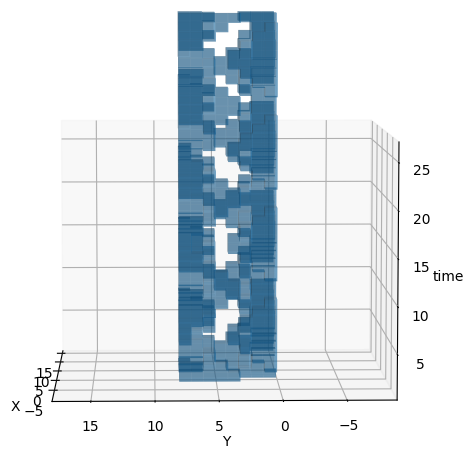
\includegraphics[width=0.7\linewidth]{example_cubical_complex.png}
  \caption{Free cubical complex of the example configuration (shown in Figure \ref{fig:example}).}
  \label{fig:example_cub_complex}
\end{figure}


\subsection{Computing evasion paths}

Once the cubical complex $F$ is obtained,
we collapse it into a graph (1-dimensional complex) $G$ in a way that preserves $H_1(F)$.
A proper elementary collapse would have to preserve higher-dimensional homology as well, however we are only interested in $H_1(F)$.
Incidentally, $F$ shouldn't have any $H_2$ generators (enclosed caves) in the case of continuous sensor movement; this would imply there is something homeomorphic to a ball in the covered complex, meaning at some time $t_0$ one or more sensors appear out of thin air, and then disappear into a point at time $t_1 > t_0$.
% TODO: proof that H_1 (and H_0) is preserved?

The vertices of $G$ correspond to connected components (by 4-connectivity) of $F$ at each time interval $[t, t + 1)$, $0 \leq t < p$.
The idea is that an intruder with unbounded speed can move between any pair of points in a connected component of free space within a finite time interval without being detected.
The vertices are labeled with $(t, c)$ where $c$ is the index of the connected component in this time slice,
and they also hold information about the area they cover (so that we can obtain concrete \texttt{Position}s after computing a cycle).

Edges in $G$ allow the intruder to move forward in time, so an edge from $(t, c)$ to $(t + 1, c')$ is added {\it iff} the connected areas $c$ and $c'$ intersect (and thus the intruder can move from $c$ to $c'$ in one time step).
If we wanted to strictly follow the homology approach to this problem, these edges would need to be undirected so we end up with a simplicial complex on which to compute $H_1$.
But in order to avoid having to filter out cycles that don't go forward in time, we kept track of the direction of edges in $G$.

\begin{figure}[H]
  \centering
  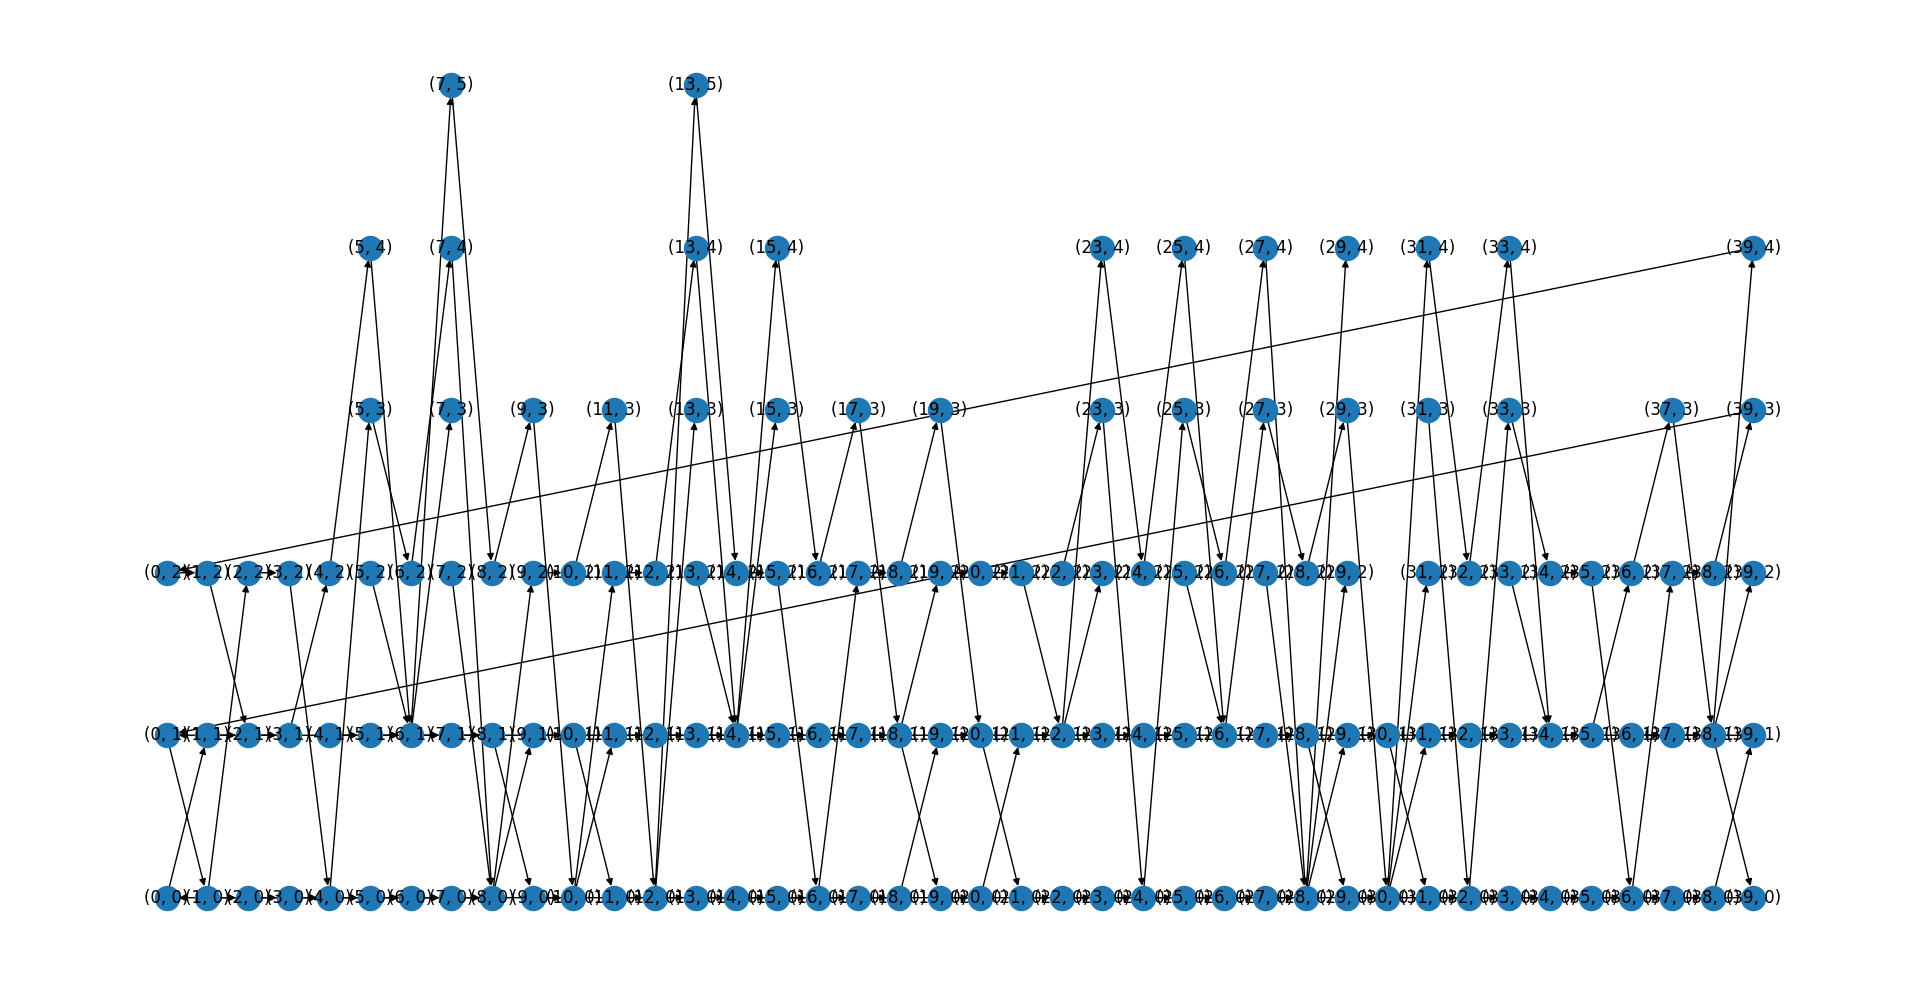
\includegraphics[width=\linewidth]{example_graph.png}
  \caption{Evasion graph $G$ of example sensor configuration (shown in Figure \ref{fig:example}).}
  \label{fig:example_graph}
\end{figure}

Cycles of $G$ are then obtained by performing a depth-first search (with depth limited to $p$) on the graph and checking whether the current node is equal to the starting node.
The above construction guarantees that each cycle in $G$ corresponds to a valid evasion path of length $p$.


\section{Results}

We tested the algorithm with several configurations.
The first configuration is trivial: a single sensor moving in the counter-clockwise direction (Figure \ref{fig:ccw}).
\begin{figure}[H]
  \centering
  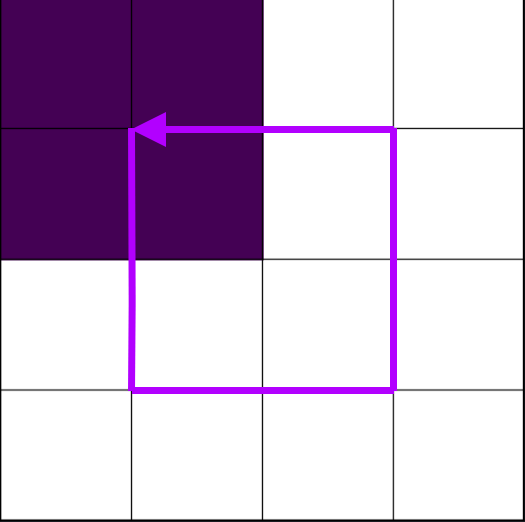
\includegraphics[width=0.7\linewidth]{ccw.png}
  \caption{Counter-clockwise circular sensor in 4x4 room, period: 8}
  \label{fig:ccw}
\end{figure}

The algorithm correctly found 1 evasion path, an animation of which can be found \href{https://github.com/MOj0/TDA_Evasion/blob/main/report/ccw.gif}{here}.

\bigskip

The next configuration is the example from the instructions (Figure \ref{fig:example}).
\begin{figure}[H]
  \centering
  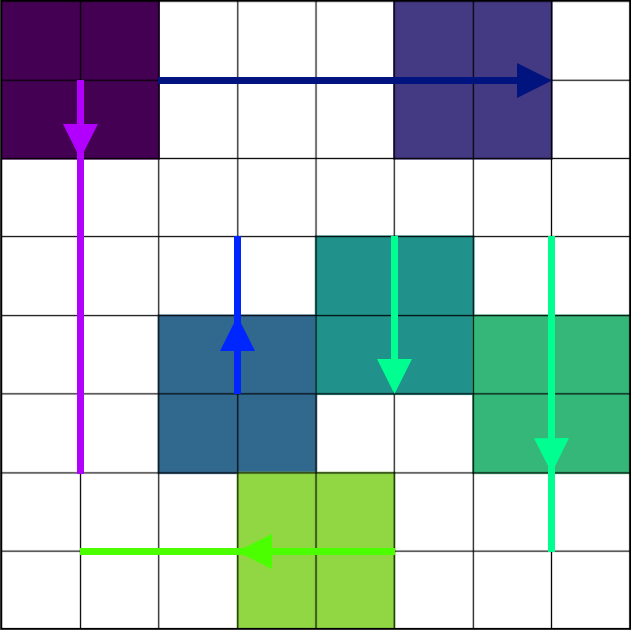
\includegraphics[width=0.7\linewidth]{example.png}
  \caption{6 sensors in 8x8 room, period: 40}
  \label{fig:example}
\end{figure}

The algorithm found 288 different evasion paths through components of free space; an animation of one path can be found \href{https://github.com/MOj0/TDA_Evasion/blob/main/report/example.gif}{here}.

\bigskip

Lastly, we tested the algorithm on random inputs, such that every point in the room is covered by at least one sensor at least part of the time.
Here are some inputs, along with their animations:

\begin{itemize}
  \item $10 \times 13$ room with 30 sensors, and a period of 80, where the algorithm found a single evasion path; an animation of the path can be found \href{https://github.com/MOj0/TDA_Evasion/blob/main/report/random_sensor_network_10x13_s30_p80_e1.gif}{here}.
  \item $12 \times 18$ room with 48 sensors, and a period of 56, where the algorithm found 2 evasion paths; an animation of one path can be found \href{https://github.com/MOj0/TDA_Evasion/blob/main/report/random_sensor_network_12x18_s48_p56_e2.gif}{here}.
  \item $12 \times 24$ room with 58 sensors, and a period of 84, where the algorithm found 68 evasion paths; an animation of one path can be found \href{https://github.com/MOj0/TDA_Evasion/blob/main/report/random_sensor_network_12x24_s58_p84_e68.gif}{here}.
  \item $20 \times 18$ room with 66 sensors, and a period of 80, where the algorithm found 247125 evasion paths; an animation of one path can be found \href{https://github.com/MOj0/TDA_Evasion/blob/main/report/random_sensor_network_20x18_s66_p80_e247125.gif}{here}.
\end{itemize}


\section{Discussion}

We implemented evasion path detection by using the cubical complex structure, reducing it to a graph and finding the cycles there.
This is equivalent to computing the $ H_1(F, \mathbb{Z})$ on the free complex, however this way we did not need to handle edge cases as described.

We also implemented paths formed of arbitrary line segments, for the sensors to follow and an algorithm that returns areas of random sizes and sensor configurations.
Lastly, we implemented animations of evasion paths as well, which help to visually confirm whether the algorithm works or not.

There is however, another limitation, considering all the assumptions made, left out to be discussed here.
Since we only allow axis-aligned cuboids in the \texttt{CubicalComplex} (ie. no diagonal edges), the algorithm is not able to detect \textit{tight} evasions.
A tight evasion is an evasion, where the object trying to escape should always be positioned on a free cell, which will be covered on the next time step.
This is a limitation of the \texttt{CubicalComplex} in the gudhi library, so if we were to do this, we would have to use another library for the data strucre.
Furthermore, the algorithm for collapsing the complex to a graph should be changed, such that the nodes of the graph are in time slices, instead of time intervals, and edges are spanned through intervals.
Since this is a limitation of the gudhi library, we decided not to implement it, as it would require too many changes.

\subsection*{Alternative approaches}

An alternative approach would subdivide the cubical complex into a simplicial one (dividing squares into triangles and cubes into tetrahedra) and computing $H_1$ generators with standard TDA software (e.g. dionysus).

A completely different approach would be to represent the time-varying (2-dimensional) free space with a zig-zag filtration and derive evasion paths from zig-zag persistence information \cite{Adams_2014}.


\section{Bibliography}

\printbibliography

\end{document}